%Plantilla Memoria Técnica:
%Modificada por: Brenda Mariana Casillas González
%Última Modificación: 02-01-2023

%------------------------------CONFIGURACION DEL DOCUMENTO

\documentclass[12pt,letterpaper,spanish]{report}
\usepackage[table]{xcolor} 
\usepackage[centertags]{amsmath}
\usepackage{amsfonts}
\usepackage{amssymb}
\usepackage{amsthm}
\usepackage[T1]{fontenc}
\usepackage[utf8]{inputenc}
\usepackage{lmodern}
\usepackage[spanish,activeacute]{babel}
% Eliminar o comentar cualquier redefinición de fuentes para evitar conflictos
% \renewcommand{\rmdefault}{lmr}
% \renewcommand{\sfdefault}{lmss}
% \renewcommand{\ttdefault}{lmtt}
\usepackage{epsfig}
\usepackage{booktabs}
\usepackage{graphicx}
\renewcommand{\baselinestretch}{1.5}
%\usepackage[numbers]{natbib}
\usepackage[round]{natbib}
\usepackage[hyphens]{url}
\usepackage{enumerate}
\usepackage{hyperref}

\newenvironment{dedication}{\newpage\large\null\em\vskip1in}%
{\vfill}

\topmargin -1 in \oddsidemargin 0in \evensidemargin 0in
\textwidth 6.5in
\textheight 9in \pagestyle{myheadings}

% -----------------------------------INICIO DEL DOCUMENTO  ---------------------------------------------------------------
\begin{document}


% Para la elaboración de esta memoria técnica se debe usar un editor profesional que soporte Latex, como recomendación se puede usar el WinEdt.

% El resultado que se sube a la plataforma debe ser en formato PDF

% Es importante mencionar que la redacción de este documento se debe hacer en tercera persona, cuidando escrupulosamente la ortografía, redacción y contenido, evitando el uso y abuso de adjetivos.

    
% ----------------------------------- CONTRAPORTADA -------------------------------------------------------------------------
%Se deben modificar los datos de la empresa, proyecto, asesores y alumnos

\thispagestyle{empty}

\begin{table}[ht]
  \centering
    \begin{tabular}{rr}
        \begin{minipage}[b]{0.05\linewidth}
        \hbox{\psfig{file=LogoUTZMG.jpg,height=1in,width=.8in}}
        \end{minipage}
    &
    \begin{minipage}[b]{.8\linewidth}
        \begin{center}
            \large{UNIVERSIDAD TECNOLÓGICA \\ DE LA ZONA METROPOLITANA DE GUADALAJARA}\\
        \end{center}
    \end{minipage}

    \end{tabular}%
\end{table}%

\begin{center}

\large{\textbf{MEMORIA TÉCNICA REALIZADA EN:}}
 \\  Corporativo Textil JSN, S. de R.L de C.V

%%Logo de la empresa
\centerline{\hbox{\psfig{file=LogoJASANA.png,height=0.4in,width=1.2in}}}

\large{\textbf{PROYECTO:} Módulo de Gestión de Reprocesos y Reposiciones}

\vspace{0.1in}
\large{\textbf{PARA OBTENER EL GRADO DE:}}

\large{Técnico Superior Universitario (TSU) en:}
\vspace{0.05in}

\large{TECNOLOGÍAS DE LA INFORMACIÓN, ÁREA DESARROLLO DE SOFTWARE MULTIPLATAFORMA }
\\
\large{PRESENTADO POR:}


Víctor Manuel Montaño Juanpedro %(Empezando con el nombre  y después apellidos)


Eduardo Isa'ias V'azquez Solís %(Empezando con el nombre  y después apellidos)

\vspace{0.2in}

\begin{tabular}{cc}
    \vspace{0.5in}
    \textbf{ASESOR INDUSTRIAL} & \textbf{ASESOR ACADÉMICO} \\

    Jair Efra'in Barragan Gárcia & Lizbeth Noriega Gútierrez \\
    \multicolumn{2}{c}{\textbf{COORDINADOR DE CARRERA}
    \vspace{0.4in}
    } \\

    \multicolumn{2}{c}{
            Mtra. Lizbeth Noriega Gutierrez }
    \end{tabular}

\end{center}
%\vspace{0.1in}
\begin{flushright}\small{ TLAJOMULCO DE ZÚÑIGA, JALISCO, AGOSTO DEL 2025} \end{flushright}

\newpage


% ------------------------------  PORTADA -----------------------------------------------------
%Se deben modificar los datos de la empresa, proyecto y alumnos


\thispagestyle{empty}


\begin{center}

 \begin{minipage}[b]{.9\linewidth}
    \begin{center}
        \vspace{0.2in}
        \large{UNIVERSIDAD TECNOLÓGICA DE LA ZONA \\METROPOLITANA DE GUADALAJARA}\\
        \large{DIRECCIÓN DE DESARROLLO Y GESTIÓN DE SOFTWARE}\\
    \end{center}
\end{minipage}
\vspace{0.3in}


\centerline{\hbox{\psfig{file=logoUTZMG.jpg,height=2in,width=1.5in}}}

\LARGE{\textsc{Módulo de Gestión de Reprocesos y Reposiciones}}
% \LARGE{\textbf{Módulo de Gestión de Reprocesos y Reposiciones}} % Alternative: bold only, no small caps

\vspace{0.2in}
\large{\textbf{MEMORIA TÉCNICA REALIZADA EN:}}
 \\  \textsc{Corporativo Textil JSN, S. de R.L de C.V}

\vspace{0.2in}
\large{\textbf{PARA OBTENER EL GRADO DE:}}

\large{Técnico Superior Universitario (TSU) en:}


\large{TECNOLOGÍAS DE LA INFORMACIÓN\\Área, DESARROLLO DE SOFTWARE MULTIPLATAFORMA }
\\

\vspace{0.2in}
\large{PRESENTADO POR:}


\textsc{Víctor Manuel Montaño Juanpedro}  %(Empezando con el nombre  y después apellidos)


\textsc{Eduardo Isaías Vázquez Solís}  %(Empezando con el nombre  y después apellidos)

\vspace{0.2in}
\small{ AGOSTO 2025}
\end{center}
%\vspace{0.1in}


\newpage



% -------------------------------------- DEDICATORIA   ---------------------
% Esta sección es opcional, pero se recomienda que se ponga, se puede redactar hasta el final y tratar que no sea mayor a una cuartilla.

        \thispagestyle{empty}
        \addcontentsline{toc}{chapter}{Agradecimientos}

        \begin{dedication}
           Agradezco a todas las personas .... Agradezco a todas las personas ....
%           A Toreto, a mi familia, a mis amigos, a mis profesores, a mi perro, a mi gato, a mi hamster, a mi pez, a mi tortuga y a todos los que me apoyaron en este proyecto.
%           Agradezco a mi familia por su apoyo incondicional, a mis amigos por su compañía y motivación, y a mis profesores por su dedicación y enseñanza.
%           A la abuelita de caperucita roja por su sabiduría y consejos, a la tortuga por su paciencia y perseverancia, y al lobo por su astucia y determinación.
%           Agradezco a todos los que me han apoyado en este proyecto, a los que me han dado su tiempo, su conocimiento y su experiencia.
%           Agradezco a Shrek por su amistad y lealtad, a Fiona por su amor y apoyo, y a Burro por su humor y alegría.
%           Tambien a mamá coco y a mamá Himelda.
%
%
%           Y y y y diles que coman tierra
        \end{dedication}


%--------------------------------         ÍNDICE


\tableofcontents


% --------------------------------------- CAPÍTULOS DEL DOCUMENTO  ----------------------------------------
% ____________________________________________________________________________________

\pagenumbering{arabic}
\oddsidemargin 0.2in \textwidth 6.5in \topmargin -0.25in
\textheight 9in \pagestyle{myheadings}

\newpage

% CAPITULO INTRODUCCIÓN. Enmarca y situa el trabajo a realizar. Tiene por objeto proporcionar una visión general del documento.
%____________________________________________________________________________________________________________________


\chapter{Introducción}
\newpage


Esta es la introducción jshdjhsdjkfhsdjk kjsdlkfjskad jdhshdfsdflksk, jdfjsdhjjkdsjkf.
Esta es la introducción jshdjhsdjkfhsdjk kjsdlkfjskad jdhshdfsdflksk, jdfjsdhjjkdsjkf.
Esta es la introducción jshdjhsdjkfhsdjk kjsdlkfjskad jdhshdfsdflksk, jdfjsdhjjkdsjkf.
Esta es la introducción jshdjhsdjkfhsdjk kjsdlkfjskad jdhshdfsdflksk, jdfjsdhjjkdsjkf.
\\




Esta es la introducción jshdjhsdjkfhsdjk kjsdlkfjskad jdhshdfsdflksk, jdfjsdhjjkdsjkf.


% CAPITULO ANTECEDENTES Y DESCIPCIÓN DE LA EMPRESA. Tiene por objeto proporcionar una visión general del documento.
%____________________________________________________________________________________________________________________

\chapter{Antecedentes y Descripción de la Empresa}
\newpage



%Nota: Los puntos que siguen son una propuesta, pongan solo los puntos que apliquen en su empresa y que los permitan poner, también puede agregar otros puntos si lo cree conveniente.

\section{Ubicación}
La empresa Corporativo Textil JSN, S. de R.L de C.V se encuentra ubicada en C. Flaviano Ramos Sur 37, Centro, 45640 Tlajomulco de Zúñiga, Jal. El mapa puede ser consultado en la Figura\ref{a01}

\begin{figure}[htp]
  \centering
  \includegraphics*{mapajasana1.png}
  \caption{Ubicación de la empresa}\label{a01}
\end{figure}



% Poner la dirección y un mapa que puede salir de maps.google.com

\section{Misión}
% Misión proporcionada por la empresa, se debe modificar la redacción a tercera persona.
Proyectar la identidad empresarial de sus clientes a través de la vestimenta de sus colaboradores, considerando su comodidad. Aplica diseños en tendencia, utiliza tecnologías actualizadas y apoya a la fuerza laboral conformada por familias mexicanas.

\section{Visión}
% Visión proporcionada por la empresa, se debe modificar la redacción a tercera persona.
Consolidar una empresa transnacional en la transformación integral de textiles, estandarizando y digitalizando procesos en sus diferentes unidades de negocio para el año 2030.

\section{Organigrama}
% Poner el organigrama proporcionado por la empresa o crear uno en caso de no contar con el.
A continuación en la figura \ref{a2} se presenta el organigrama de la empresa.

\begin{figure}[htp]
  \centering
  \includegraphics[width=\linewidth]{Organigrama_Jasana3.png}
  \caption{Organigrama de Textil JSN}\label{a2}
\end{figure}

\section{Historia}
En corporativo textil jsn, diseñamos y creamos prendas y textiles para hoteles y empresas de hospitalidad.
Nos dedicamos a que los colaboradores de nuestros clientes estén presentables y cómodos todos los días, priorizando su seguridad e integridad.
Esto lo logramos incorporando tecnologías en nuestras prendas que además aumentan su vida útil.


\newpage

% --------------------------------   CAPITULO PROBLEMÁTICA   --------------------------------------
%____________________________________________________________________________________________________________________



\chapter{Problemática y Descripción del Proyecto}
\newpage

\section{Problemática}

La empresa \textbf{Corporativo Textil JSN}, dedicada a la fabricación de uniformes corporativos, enfrenta actualmente diversas dificultades en el control, trazabilidad y gestión eficiente de los \textit{reprocesos y reposiciones} de piezas defectuosas o dañadas durante la producción. Aunque se utiliza el sistema ERP (Enterprise Resource Planning) Odoo, este proceso específico no se encuentra digitalizado ni debidamente integrado al entorno operativo, generando así múltiples problemáticas en distintas áreas del flujo productivo y administrativo.

Las principales problemáticas detectadas son las siguientes:

\begin{enumerate}
    \item \textbf{Falta de trazabilidad:} No existe un registro digital estandarizado de qué piezas fueron reprocesadas, cuándo, por quién, ni en qué etapa del proceso ocurrieron los daños.
    
    \item \textbf{Procesos manuales:} Actualmente, la información relacionada con daños, responsables y tiempos de corrección se gestiona mediante hojas físicas, lo cual incrementa el riesgo de pérdida de información y errores humanos.
    
    \item \textbf{Descontrol en la gestión por áreas:} Las distintas áreas involucradas en la producción (Diseño, Corte, Ensamble, Planchado, entre otras) operan de forma aislada en cuanto al manejo de reprocesos, sin un sistema común que garantice la continuidad y visibilidad del flujo entre ellas.
    
    \item \textbf{Dificultad para calcular tiempos y costos:} No se cuenta con una herramienta que permita realizar cálculos automáticos del tiempo invertido en cada reproceso, ni estimaciones precisas del costo de materiales e insumos reinvertidos.

\end{enumerate}

Ante este panorama, se vuelve indispensable el desarrollo de una solución digital que permita sistematizar la gestión de reprocesos y reposiciones, garantizando control, transparencia, eficiencia operativa y toma de decisiones basada en información precisa y actualizada

% En esta sección se deberá redactar un planteamiento de la problemática que se pretende resolver.


%Escribir un resumen de su proyecto en donde se hable del aspecto económico, operativo, técnico, humano, objetivos, etc.
\section{Descripción del Proyecto}

El proyecto se basa en el diseño y desarrollo de una herramienta a medida que permita gestionar de forma centralizada, digital y trazable los procesos de reposición y reproceso de piezas defectuosas en la cadena de producción de la empresa Corporativo Textil JSN.

A diferencia de un módulo integrado, esta aplicación funcionará de manera independiente al ERP Odoo que la empresa utiliza para otras operaciones dado a restricciones del propio ERP y cuestiones a nivel operacional dentro de la empresa, facilitando así una mayor flexibilidad en el desarrollo y una interfaz de usuario especializada para esta tarea. El sistema se construirá utilizando tecnologías web modernas, tales como \textbf{React} para el desarrollo de la interfaz de usuario.

La aplicación web implementará las siguientes características clave para resolver la problemática:
\begin{itemize}
    \item \textbf{Registro centralizado de solicitudes:} Gestión de todos los casos de reproceso y reposición con folios únicos para un seguimiento preciso.
    \item \textbf{Asignación de responsabilidades por área:} Flujos de trabajo que permiten asignar tareas y notificar a las áreas correspondientes (Diseño, Corte, Ensamble, etc.).
    \item \textbf{Cálculo automático de tiempos y costos:} Herramientas para registrar el tiempo invertido y los materiales utilizados en cada corrección.
    \item \textbf{Generación de reportes históricos:} Creación de informes y estadísticas para analizar tendencias, identificar cuellos de botella y fundamentar la toma de decisiones.
\end{itemize}

\subsubsection{Objetivo General}
\label{sec:objetivo_general}

Desarrollar e implementar una herramienta que permita gestionar digitalmente las solicitudes de reproceso y reposición de la empresa, asegurando la trazabilidad del proceso, el control por área y la generación de reportes históricos para la toma de decisiones.

\subsubsection{Objetivos Específicos}
\label{sec:objetivos_especificos}

\begin{itemize}
    \item Permitir el registro eficiente de solicitudes con folios y datos clave de producción.
    \item Asignar y seguir responsabilidades por área en el flujo del reproceso.
    \item Automatizar el cálculo de tiempos de reproceso y sus costos estimados.
    \item Generar reportes que ayuden en el análisis.
\end{itemize}


%Describir de manera detallada las actividades para el desarrollo de la estadía y/o proyecto (Diagrama de Gantt).
\subsection{Planeación}

Por cuestiones de organización y aprovechamiento eficiente del tiempo que se tiene previsto para realizar el proyectó se ha desarrollado un plan de trabajo estructurado mediante un diagrama Gantt, el cual nos facilita una mejor gestión del tiempo creando una ayuda visual para las actividades, plazos, fases clave y progreso planeados en el desarrollo de este módulo. El conjunto de las siguientes imágenes (\ref{a03} a \ref{a05}) muestra una vista general de las actividades planeadas con sus respectivos espacios de tiempo y recursos

\begin{figure}[htp]
  \centering
  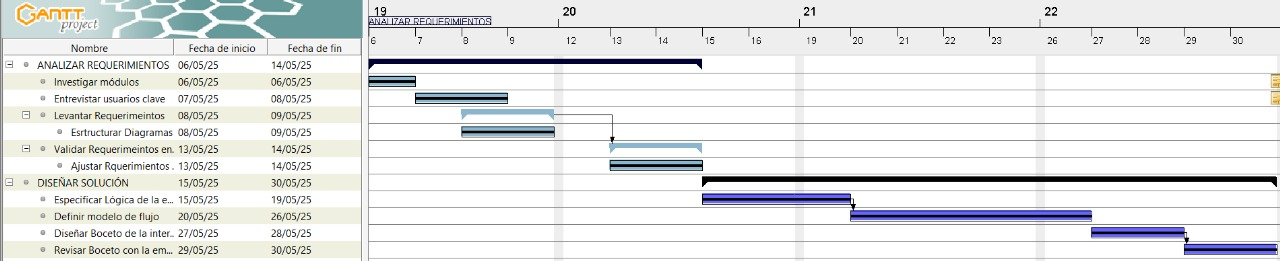
\includegraphics[width=0.9\textwidth]{Gantt_Mayo_30.jpg}
  \caption{Actividades correspondientes a Mayo}\label{a03}
\end{figure}

\begin{figure}[htp]
  \centering
  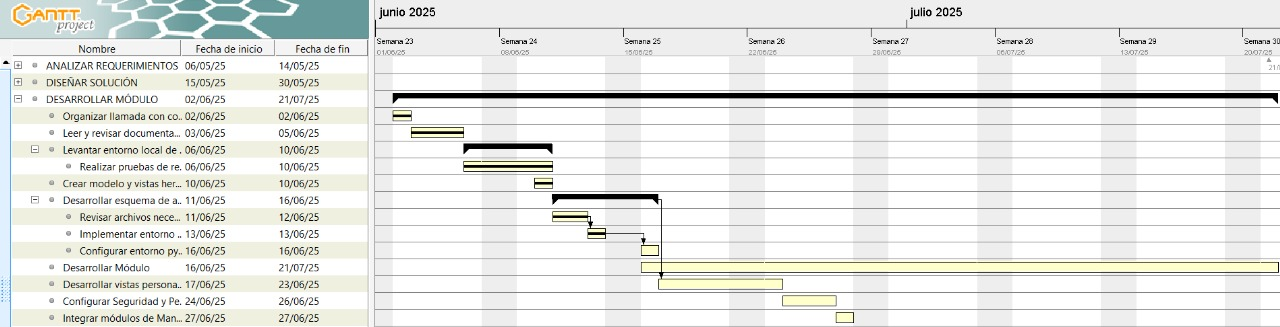
\includegraphics[width=0.9\textwidth]{Gantt_Week_23_30.jpg}
  \caption{Periodo correspondiente a Junio-Julio}\label{a04}
\end{figure}

\begin{figure}[htp]
  \centering
  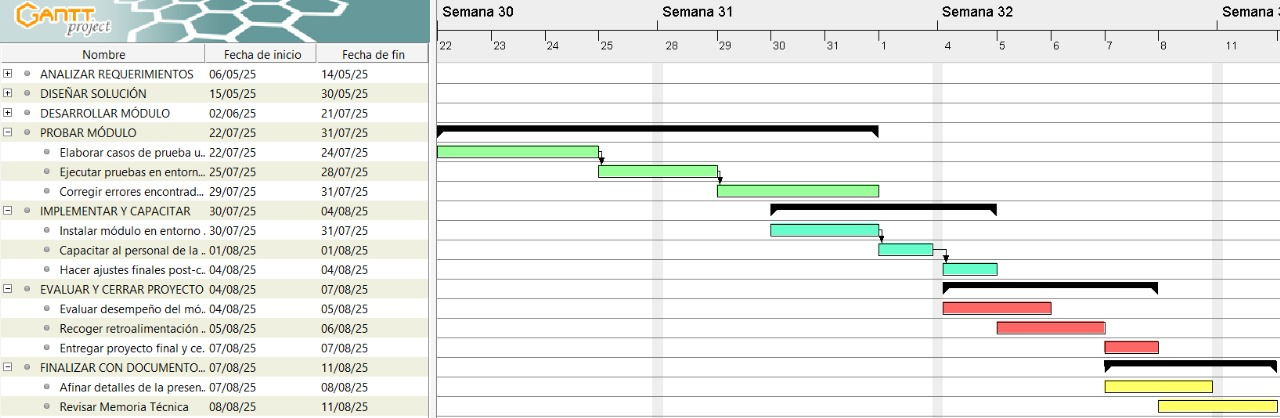
\includegraphics[width=0.9\textwidth]{Gantt_Week_30_32.jpg}
  \caption{Periodo correspondiente a Julio-Agosto}\label{a05}
\end{figure}
%CAPITULO MARCO TEÓRICO: bases teorícas del proyecto. conceptos básicos y antecedentes o información existente.
%____________________________________________________________________________________________________________________

\chapter{Marco Teórico}
\newpage

\section{Sistemas ERP}
Un sistema de Planificación de Recursos Empresariales (ERP) es mucho más que una simple herramienta tecnológica; se define como un sistema integrado que optimiza los procesos de negocio, abarcando desde la gestión financiera y de recursos humanos hasta la logística y la producción \citep{Hammouch_2024}. Esta integración holística tiene como objetivo principal mejorar tanto la visibilidad de las operaciones como la eficiencia operativa, que son elementos cruciales en la gestión moderna.

La función principal de un ERP es gestionar los procesos de negocio centrales de una compañía en tiempo real, combinando diversas funciones en un único sistema unificado. Al centralizar los datos y agilizar las operaciones, los sistemas ERP conducen a una mayor eficiencia y facilitan una toma de decisiones más informada \cite{Hammouch_2024}.

%Durante los últimos años el mercado tecnológico ha avanzado de manera extraordinaria implantándose en otros ámbitos como los negocios, añadiéndole un nuevo valor a la información que se vuelve necesaria para el análisis y la toma de decisiones. Este es el motivo por el cual cada vez más empresas están considerando la implementación de un sistema ERP en su proceso de producción a manera de sistema central para el manejo y gestión de sus recursos, entrando de esta forma a competir en el siempre creciente e innovador mercado tecnológico e informático. 

\subsubsection{El Legado de los Silos y la Evolución hacia la Integración}

Históricamente, la mayoría de las empresas operaban con sistemas de información no integrados que soportaban únicamente las actividades de áreas funcionales individuales \cite{book}. Esto significaba que una compañía podía tener un sistema de información para marketing, otro para producción y así sucesivamente, cada uno con su propio hardware, software y métodos para procesar los datos. A esta configuración se le conoce como \textbf{silos} o \textit{stovepipes}, ya que cada departamento poseía su propia pila de información, desconectada de las demás, lo que generaba ineficiencias significativas y falta de coordinación \cite{book}.

La transición desde este modelo de silos hacia los sistemas integrados que hoy conocemos como ERP no fue repentina, sino una evolución gradual impulsada por la confluencia de varios factores clave. El surgimiento de los sistemas ERP actuales fue el resultado de tres elementos principales: (1) el avance de la tecnología de hardware y software, (2) el desarrollo de una visión de sistemas de información integrados, y (3) la reingeniería de las empresas para pasar de un enfoque funcional a uno centrado en los procesos de negocio \cite{book}.

\subsection{Las raíces en la manufactura: MRP y MRP II}
%Los orígenes de los sistemas integrados se encuentran, efectivamente, en el sector de la manufactura, y el concepto tomó forma en la planta de producción . El software de manufactura avanzó significativamente durante las décadas de 1960 y 1970, evolucionando desde simples sistemas de seguimiento de inventario hasta el software de **Planificación de Requerimientos de Materiales (MRP)**.
%
%Formalmente, MRP es una metodología de programación de la producción que determina el tiempo y la cantidad de las corridas de producción y de las órdenes de compra para cumplir con un programa maestro de producción . En la práctica, el software MRP permitía a un gerente de planta planificar la producción y los requerimientos de materias primas trabajando en retrospectiva a partir del pronóstico de ventas, prediciendo así la demanda futura. Aunque los sistemas MRP básicos podían funcionar en computadoras mainframe, fue la llegada del intercambio electrónico de datos (EDI) lo que permitió a las empresas manejar el proceso de compras de manera electrónica, sentando las bases para la gestión de la cadena de suministro \citep{}.
%
%En la década de los 80, estos sistemas evolucionaron hacia la Planificación de Recursos de Manufactura (MRP II). A diferencia del MRP original, el MRP II integraba no solo los materiales, sino también los recursos de la planta y la mano de obra, incorporando funcionalidades de planificación de capacidad y finanzas. MRP II fue un paso crucial hacia la integración, ya que comenzaba a coordinar diferentes áreas del ciclo de producción dentro de un marco unificado.

Los orígenes de los sistemas de planificación de recursos empresariales se encuentran en el sector de la manufactura, donde la necesidad de gestionar eficientemente los materiales dio lugar a las primeras metodologías de planificación \citep{book,Miño-Cascante_Saumell-Fonseca_Toledo-Borrego_Roldan-Ruenes_Moreno-García_2015}. Durante las décadas de 1960 y 1970, el aumento de la capacidad de cómputo permitió la creación de los primeros sistemas de \textbf{Planificación de Requerimientos de Materiales (MRP)}, cuyo objetivo era calcular las necesidades de materias primas y las fechas de sus pedidos para cumplir con los planes de producción, asegurando la disponibilidad de materiales y reduciendo los costos de inventario \citep{book}.

Posteriormente, estos sistemas evolucionaron hacia una planificación más integral. Esta evolución es descrita como \textbf{Planificación de Recursos de Manufactura (MRP II)}, un concepto que, a diferencia del MRP original, integraba no solo los materiales, sino también las capacidades productivas de la planta, los recursos monetarios y el personal \citep{Miño-Cascante_Saumell-Fonseca_Toledo-Borrego_Roldan-Ruenes_Moreno-García_2015}. El MRP II fue un paso crucial hacia la integración, ya que comenzaba a coordinar diferentes áreas del ciclo de producción dentro de un marco unificado, sentando las bases para los futuros sistemas ERP \citep{Miño-Cascante_Saumell-Fonseca_Toledo-Borrego_Roldan-Ruenes_Moreno-García_2015}.


\subsection{Los motores del cambio en los años 90}
El verdadero nacimiento de los sistemas ERP, tal como los conocemos hoy, ocurrió a principios de los años 90, ya que los sistemas de hardware y software no fueron lo suficientemente complejos y potentes para soportarlos hasta esa década. Esta transición fue posible gracias a la confluencia de tres factores clave: el avance de la tecnología, el desarrollo de una visión de sistemas integrados y la reingeniería de las empresas hacia un enfoque en procesos \cite{book}.

\paragraph{Avances tecnológicos} La Ley de Moore describía el crecimiento exponencial del poder de cómputo, lo que hacía que el hardware fuera cada vez más potente y asequible. Crucialmente, la industria se movió de la costosa arquitectura \textit{mainframe} a la más flexible y distribuida arquitectura cliente-servidor. Al mismo tiempo, el desarrollo y madurez de los sistemas de gestión de bases de datos relacionales (DBMS) durante los años 70 y 80 proporcionaron la tecnología necesaria para construir una base de datos centralizada y compartida \cite{book}.

\paragraph{La visión de la integración} En el ámbito empresarial, las duras condiciones económicas de finales de los 80 y principios de los 90 impulsaron a las empresas a buscar una mayor eficiencia a través de la reorganización. Conceptos como la \textbf{Reingeniería de Procesos de Negocio (BPR)}, popularizados por autores como Michael Hammer, promovieron la idea de rediseñar radicalmente los procesos de negocio. Esto creó el ambiente perfecto para que los gerentes comenzaran a ver el software ERP como una solución a los problemas de negocio \cite{book}.

\paragraph{El surgimiento de SAP} La compañía alemana SAP, fundada en 1972 por ex-empleados de IBM, fue la pionera en materializar esta visión. En 1992, SAP lanzó su revolucionario software \textbf{R/3}, diseñado específicamente para la arquitectura cliente-servidor. Este sistema permitía a las empresas conectar sus diferentes áreas funcionales a una única base de datos subyacente, ofreciendo una solución integrada en tiempo real, lo que sentó las bases para el mercado ERP moderno \cite{book}.

\paragraph{El catalizador del Y2K y la expansión del mercado} Un evento inesperado aceleró masivamente la adopción de los sistemas ERP a finales de los 90: el \textbf{problema del año 2000 (Y2K)}. Muchas empresas utilizaban sistemas heredados (\textit{legacy systems}) que almacenaban el año con solo dos dígitos y se enfrentaron a la decisión de reparar estos sistemas obsoletos o reemplazarlos por completo con una solución moderna e integrada. Muchas eligieron la segunda opción, lo que provocó un auge sin precedentes en las ventas de ERP, periodo durante el cual competidores como Oracle y PeopleSoft también ganaron una cuota de mercado significativa \cite{book}.

A partir del nuevo milenio, los sistemas ERP continuaron evolucionando, incorporando funcionalidades de gestión de la relación con el cliente (CRM) y de la cadena de suministro (SCM), y adaptándose a nuevas tecnologías como el cómputo en la nube, el software como servicio (SaaS) y la movilidad \cite{book}.


\section{Antecedentes y trabajos previos:}
\label{sec:antecedentes}

Para contextualizar la presente investigación y fundamentar su relevancia, es imprescindible revisar trabajos anteriores que aborden problemáticas similares o que exploren el uso de las tecnologías propuestas. A continuación, se analizan dos trabajos de investigación recientes que sirven como antecedentes directos y técnicos para el desarrollo de esta propuesta: un proyecto de mejora de la gestión docente en una universidad pública utilizando Odoo y un desarrollo técnico de una aplicación específica sobre la misma plataforma.

\subsection{Antecedente en la gestión de procesos docentes universitarios}
\label{sub:antecedente_gestion_docente}

Un antecedente de alta relevancia es el trabajo de investigación de maestría titulado \textit{Propuesta de mejora para el proceso de gestión docente de la 
Universidad Nacional Autónoma de Chota, 2024} en la Escuela de Posgrado Newman, Perú. Este estudio aborda una problemática directamente análoga a la de la presente tesis, explorando la situación de una universidad pública con el objetivo de proponer una solución tecnológica que mejore sus procesos de gestión docente.
%\citep{pretell2024mejora}
El autor identifica que, en el contexto de las universidades públicas, existen carencias y limitaciones en los procesos académicos, especialmente los referidos a la gestión docente. Estos procesos incluyen el reclutamiento y selección, la inducción, la formación continua, la evaluación del desempeño y el reconocimiento docente. La investigación de Pretell Cruzado tuvo como resultado el diseño y la validación del software ERP Odoo v.17 - edición Community como la solución tecnológica a implementar para sistematizar dichos procesos. La conclusión de su trabajo afirma que una solución de este tipo ofrece beneficios tangibles en el marco de la transformación digital, como un mejor acceso en línea a la información, mayor transparencia y la optimización general del proceso de gestión docente.

Este trabajo es fundamental como antecedente, ya que valida tanto la problemática abordada como la elección de Odoo ERP como una herramienta tecnológica viable y pertinente para mejorar la gestión docente en el ámbito universitario público.

\subsection{Antecedente en el desarrollo de interfaces modernas en Odoo}
\label{sub:antecedente_desarrollo_tecnico}

Desde una perspectiva técnica, el trabajo de fin de grado  \textit{Desarrollo de una Aplicación en el sistema de código abierto Odoo para la Gestión de Residencias \citep{TortCarrillo2024}}, sirve como un excelente referente. Aunque el dominio de aplicación es distinto (residencias geriátricas), su enfoque se centra en el desarrollo de una interfaz de usuario (UI) moderna sobre la plataforma Odoo.

El objetivo principal del proyecto fue la creación de una interfaz de usuario intuitiva y adaptable, utilizando específicamente el framework de JavaScript \textbf{Odoo Web Library (OWL)}. OWL es descrito como una herramienta moderna y eficiente para la creación de aplicaciones web reactivas dentro del ecosistema de Odoo. Este antecedente es técnicamente relevante porque demuestra la capacidad de Odoo para ir más allá de sus interfaces estándar, permitiendo la construcción de soluciones visuales a medida para necesidades específicas.

Asimismo, el trabajo subraya la importancia de la integración del nuevo módulo con otros módulos preexistentes en Odoo para asegurar una gestión correcta del flujo de información. Por lo tanto, este estudio valida el uso de las herramientas de frontend más modernas de Odoo (OWL) para la creación de aplicaciones especializadas y destaca la arquitectura modular e integrada de la plataforma.




\section{Arquitectura y componentes de sistemas ERP:}

La arquitectura de un sistema ERP define su estructura técnica, su funcionamiento y su capacidad de adaptación. Para comprender la diversidad de enfoques en el mercado, este capítulo realiza un análisis comparativo entre dos sistemas paradigmáticos: SAP, como representante del modelo de ERP tradicional y líder del mercado, y Odoo, como exponente de los sistemas ERP modernos de código abierto.

\subsection{Modelo de negocio y licenciamiento}


El modelo de negocio dicta cómo una empresa adquiere, implementa y mantiene su sistema ERP, lo cual tiene un impacto directo en el costo total de propiedad (TCO).

\paragraph{SAP (Modelo Propietario Tradicional)}
SAP opera bajo un modelo de software propietario y de código cerrado. Históricamente, esto implica costos significativos asociados a la adquisición de licencias de software, honorarios de consultores certificados para la implementación y contratos de mantenimiento anual para recibir soporte y actualizaciones. Este modelo, aunque costoso, ofrece a las grandes corporaciones un ecosistema robusto y un soporte centralizado.

\paragraph{Odoo (Modelo \textit{Open Core})}
En contraposición, Odoo se presenta como una plataforma de planificación de recursos empresariales de código abierto \cite{pretell2024mejora} que opera bajo un modelo de negocio conocido como ``Open Core''. Este modelo se manifiesta en dos versiones principales, permitiendo una gran flexibilidad para las organizaciones \cite{TortCarrillo2024}:
\begin{enumerate}
    \item \textbf{Odoo Community:} Es la versión gratuita y de código abierto, mantenida gracias a una comunidad global de desarrolladores.
    \item \textbf{Odoo Enterprise:} Es la versión comercial de pago, que funciona bajo un modelo de suscripción e incluye funcionalidades adicionales y servicios de soporte directo del fabricante.
\end{enumerate}
Este modelo dual ofrece un punto de entrada de bajo costo para las empresas, especialmente para las PyMEs, y una ruta de escalamiento hacia una solución más robusta y soportada a medida que estas crecen.

\subsection{Arquitectura tecnológica}

La pila tecnológica (o \textit{stack}) define los componentes de software y lenguajes sobre los que se construye el sistema.

\paragraph{SAP (Arquitectura Cliente-Servidor y Lenguaje Propietario)}
El éxito de SAP se fundamentó en su arquitectura cliente-servidor de tres capas: presentación (SAP GUI), aplicación y base de datos. El desarrollo y la personalización se realizan utilizando su propio lenguaje de programación patentado, \textbf{ABAP (Advanced Business Application Programming)}.

\paragraph{Odoo (Arquitectura Web y Pila de Código Abierto)}
Odoo está construido sobre una pila tecnológica moderna y de código abierto, diseñada para ser nativa de la web. Su arquitectura también sigue un modelo de tres capas:
\begin{enumerate}
    \item \textbf{Base de Datos:} Utiliza exclusivamente \textbf{PostgreSQL}.
    \item \textbf{Servidor (Lógica):} El núcleo está escrito en \textbf{Python} y cuenta con un potente \textbf{ORM (Mapeo Objeto-Relacional)} que facilita el desarrollo.
    \item \textbf{Cliente (Presentación):} La interfaz es un cliente web moderno donde las vistas se definen con \textbf{XML} y la interactividad con \textbf{JavaScript}.
\end{enumerate}

\subsection{Modularidad y cobertura funcional}

\paragraph{SAP (Módulos Funcionales Clásicos)}
SAP estructura su sistema en un conjunto de módulos funcionales altamente integrados pero bien definidos, que corresponden a las áreas clásicas de una gran empresa: \textbf{SD} (Ventas y Distribución), \textbf{MM} (Gestión de Materiales), \textbf{PP} (Planificación de la Producción), \textbf{FI} (Contabilidad Financiera), \textbf{CO} (Controlling) y \textbf{HR} (Recursos Humanos).

\paragraph{Odoo (Enfoque basado en ``Apps'')}
Odoo adopta un enfoque hiper-modular, organizando su funcionalidad en ``Apps'' que se pueden instalar o desinstalar fácilmente. Las aplicaciones principales se corresponden directamente con los módulos clásicos de SAP:
\begin{itemize}
    \item La App \textbf{Ventas} de Odoo es el análogo funcional de \textbf{SAP SD}.
    \item Las Apps \textbf{Inventario} y \textbf{Compras} cubren las funciones de \textbf{SAP MM}.
    \item La App \textbf{Fabricación} de Odoo corresponde al módulo \textbf{SAP PP}.
    \item La App \textbf{Contabilidad} integra funcionalidades de \textbf{SAP FI y CO}.
\end{itemize}
La gran diferencia radica en su ecosistema, donde existen miles de aplicaciones adicionales para cubrir necesidades muy específicas.

\subsection{Flexibilidad y personalización}

\paragraph{SAP (Configuración vs. Personalización)}
SAP distingue claramente entre \textbf{configuración} (ajustes mediante herramientas integradas) y \textbf{personalización} (modificar el código ABAP), siendo esta última una tarea compleja, costosa y que puede dificultar las actualizaciones del sistema.

\paragraph{Odoo (Flexibilidad a través del Código Abierto)}
La flexibilidad de Odoo es uno de sus principales argumentos de venta. La práctica estándar no es modificar el código del núcleo, sino \textbf{crear módulos personalizados} que se instalan sobre el sistema base. Estos módulos pueden añadir o alterar funcionalidades de forma segura, asegurando que el núcleo del sistema pueda ser actualizado sin afectar las personalizaciones.

\section{Desarrollo de módulos en odoo}
\label{sec:desarrollo_modulos}

Toda la funcionalidad en Odoo está organizada en \textbf{módulos}. Toda la funcionalidad en Odoo está organizada en módulos. Según la documentación oficial de Odoo \citep{odooDocs}, un módulo es técnicamente un directorio que agrupa el código y los recursos del sistema para añadir o modificar una funcionalidad específica. Esta estructura es fundamental para el desarrollo, ya que consiste en la creación o extensión de estos módulos, en lugar de modificar el código fuente del núcleo del sistema \citep{reis2022odoo}. Esta arquitectura no solo garantiza que las personalizaciones se mantengan organizadas y separadas del código fuente del núcleo, facilitando el mantenimiento y las actualizaciones, sino que también permite que el sistema sea extremadamente escalable, pudiendo activar o desactivar funcionalidades completas según las necesidades del negocio.

\subsection{Estructura fundamental de un módulo}
\label{sub:estructura_modulo}
Cada módulo de Odoo es un directorio cuyo nombre técnico es el que se utilizará para referenciarlo. Dentro de él, se encuentran archivos y subcarpetas que organizan sus componentes por convención. Una estructura completa suele incluir:
\begin{itemize}
    \item \textbf{\texttt{\_\_manifest\_\_.py}}: Es el archivo descriptor del módulo y el único estrictamente obligatorio. Contiene un diccionario de Python con metadatos clave como el nombre del módulo (\texttt{name}), versión (\texttt{version}), autor (\texttt{author}), categoría funcional (\texttt{category}), un resumen de su propósito (\texttt{summary}), y, de forma crucial, sus dependencias (\texttt{depends}), que aseguran que otros módulos necesarios se instalen primero. También define los archivos de datos, vistas y seguridad a cargar.

    \item \textbf{\texttt{models/}}: Contiene los archivos de Python (\texttt{.py}) que definen los modelos de datos y su lógica de negocio. Es el corazón del módulo.

    \item \textbf{\texttt{views/}}: Contiene los archivos XML (\texttt{.xml}) que definen la interfaz de usuario: las vistas, los menús que las invocan y las acciones que las conectan.

    \item \textbf{\texttt{controllers/}}: Alberga los archivos Python que manejan las peticiones web. Son esenciales para crear páginas para el sitio web de Odoo o para definir puntos de acceso (endpoints) para APIs RESTful personalizadas.

    \item \textbf{\texttt{security/}}: Contiene los archivos que definen los permisos de acceso. Principalmente el archivo \texttt{ir.model.access.csv}, que especifica qué grupos de usuarios pueden realizar operaciones de lectura, escritura, creación o borrado en cada modelo.

    \item \textbf{\texttt{data/}}: Contiene archivos XML utilizados para cargar datos iniciales o de configuración que el módulo necesita para funcionar, como secuencias, categorías de productos o plantillas de correo.

    \item \textbf{\texttt{static/}}: Contiene los archivos estáticos (CSS, Sass, JavaScript, imágenes, fuentes) que se usarán en la capa de presentación, tanto en el backend como en el frontend del sitio web.
\end{itemize}

\subsection{Modelos (capa de datos y lógica)}
\label{sub:modelos_odoo}
Los modelos son la columna vertebral de Odoo. Son clases de Python que heredan de \texttt{models.Model} y utilizan el \textbf{ORM (Mapeo Objeto-Relacional)} de Odoo para mapear cada clase a una tabla en la base de datos PostgreSQL y cada instancia de la clase a un registro en esa tabla. El ORM implementa un patrón de tipo \textit{Active Record}, donde los objetos llevan consigo tanto los datos como los métodos para operar sobre ellos. Esta capa es responsable de:

\begin{enumerate}
    \item \textbf{Definición de la estructura de datos:} Se definen los campos como atributos de la clase. Odoo ofrece una gran variedad de tipos de campo, desde los simples como \texttt{Char}, \texttt{Integer}, \texttt{Float}, \texttt{Date}, \texttt{Datetime}, \texttt{Boolean} y \texttt{Html}, hasta los relacionales que son clave para un ERP: \texttt{Many2one} (para claves foráneas, como vincular una factura a un cliente), \texttt{One2many} (la relación inversa, como ver todas las facturas de un cliente) y \texttt{Many2many} (para relaciones múltiples, como asignar varias etiquetas a un producto).

    \item \textbf{Implementación de la lógica de negocio:} Se escriben métodos en Python decorados para interactuar con el ORM. Decoradores como \texttt{@api.depends} permiten crear campos cuyos valores se calculan dinámicamente a partir de otros, mientras que \texttt{@api.constrains} define reglas de validación de datos a nivel de base de datos para garantizar la consistencia.

    \item \textbf{Herencia de Modelos:} Una de las características más potentes de Odoo es su mecanismo de herencia, que permite modificar modelos existentes de forma no intrusiva. Se puede extender un modelo existente para añadirle nuevos campos, modificar los atributos de campos existentes o sobreescribir sus métodos para adaptar su comportamiento a nuevas necesidades, todo sin tocar el código del módulo original.
\end{enumerate}

\subsection{Vistas (capa de presentación)}
\label{sub:vistas_odoo}
Las vistas en Odoo, definidas en \textbf{XML}, son la forma de presentar los datos de los modelos al usuario. El motor de Odoo interpreta estos archivos XML para generar dinámicamente las vistas HTML interactivas, utilizando un motor de plantillas llamado \textbf{QWeb}. Las vistas se conectan con los modelos a través de \textbf{Acciones} (\texttt{ir.actions.act\_window}), que son registros en la base de datos que definen qué vistas mostrar para un modelo particular. Los tipos de vista principales son:
\begin{itemize}
    \item \textbf{Vistas de formulario (\texttt{form}):} La vista detallada para un único registro. Su estructura puede ser altamente personalizada con elementos como pestañas, grupos y botones que ejecutan métodos del modelo.
    \item \textbf{Vistas de lista (\texttt{tree}):} Muestran múltiples registros en una tabla. Permiten la edición en línea y la visualización resumida de la información.
    \item \textbf{Vistas kanban (\texttt{kanban}):} Presentan los registros como tarjetas organizadas en columnas, ideal para visualizar flujos de trabajo basados en etapas (por ejemplo, un pipeline de ventas).
    \item \textbf{Vistas de búsqueda (\texttt{search}):} Definen los filtros, campos de búsqueda y opciones de agrupación ("Agrupar por") que el usuario puede utilizar para analizar los datos.
\end{itemize}

\subsection{Controladores y workflows}
\label{sub:controladores_workflows}
Los \textbf{Controladores} son el mecanismo para crear lógica de servidor que responda a peticiones web. Heredan de la clase \texttt{http.Controller} y sus métodos se asocian a rutas (URLs) mediante un decorador. Esto permite crear desde simples páginas web con contenido dinámico hasta complejos puntos de acceso (endpoints) de API que devuelven datos en formato JSON.

El concepto de \textbf{Workflow} ha evolucionado. En versiones antiguas de Odoo (anteriores a la 8), existía un complejo sistema de workflows basado en XML que definía los flujos de documentos. Este sistema ha sido reemplazado por un enfoque más simple y flexible implementado directamente en Python. Hoy en día, un flujo de trabajo se modela típicamente con un campo de tipo \texttt{Selection} llamado \texttt{state} en el modelo (ej: 'borrador', 'enviado', 'aprobado', 'hecho'). La transición entre estados es gestionada por métodos del modelo (ej: \texttt{def action\_confirm()}) que son llamados por botones en las vistas. Estos métodos contienen toda la lógica de negocio: cambiar el estado, crear otros registros, enviar correos, etc.

\section{Tecnologías usadas}
\label{sec:tecnologias_usadas}
La plataforma Odoo se fundamenta en un modelo de despliegue y una filosofía de desarrollo que son clave para entender su flexibilidad y alcance. Estos se basan en los conceptos de Software como Servicio (SaaS) y el uso de tecnologías de código abierto (Open Source).

\subsection{Modelo de despliegue: software como servicio (SaaS)}

Un concepto clave en la oferta de los sistemas ERP modernos es el de Software como Servicio (SaaS). Este paradigma consiste en que un proveedor ofrece acceso a aplicaciones de software a través de internet, eliminando la necesidad de que el usuario descargue, instale o actualice programas en su propio equipo \cite{dura2022saas}. Las ventajas de este enfoque son considerables, e incluyen ahorros significativos en costos relacionados con la adquisición de infraestructura de TI, mantenimiento y seguridad \cite{dura2022saas}.

Odoo ERP es un claro exponente de los programas que operan bajo el modelo SaaS, y su aplicación ha demostrado ser particularmente útil para optimizar la actividad en entidades de investigación y educación, permitiendo una transformación digital acelerada \cite{dura2022saas}.

\subsection{Filosofía de código abierto (open source)}

Además de su modelo de despliegue, Odoo se apoya en una pila tecnológica basada casi en su totalidad en tecnologías de código abierto (\textit{open source}). El software con licencia de código abierto se caracteriza por proveer un código fuente que cualquiera puede ver, usar, modificar y distribuir de manera gratuita \cite{pretell2024mejora}.

Esta elección deliberada no solo reduce los costos de licenciamiento, sino que también permite a Odoo beneficiarse de la innovación y la seguridad impulsadas por una extensa comunidad global de programadores que, de manera continua, desarrollan nuevos módulos y favorecen la adaptabilidad del sistema \cite{pretell2024mejora}.

%\subsection{Backend: Python}
%El lenguaje de programación principal para todo el desarrollo del backend en Odoo es \textbf{Python}. La elección de Python es estratégica debido a su sintaxis limpia y legible, que reduce los costos de mantenimiento, y a su vasto ecosistema de librerías de terceros. Odoo aprovecha varias de estas librerías, como \texttt{lxml} para el procesamiento de alta velocidad de los archivos XML de las vistas y \texttt{psycopg2} para la comunicación con la base de datos. El propio framework de Odoo provee toda la infraestructura necesaria, incluyendo el ORM, el motor de plantillas y el servidor web.

\subsection{Backend: Python}

El lenguaje de programación principal para todo el desarrollo del backend en Odoo es \textbf{Python}. La elección de este lenguaje es estratégica debido a su sintaxis limpia y legible, que reduce los costos de mantenimiento, y a su vasto ecosistema de librerías de terceros \cite{pythonDocs}. El propio framework de Odoo, desarrollado sobre Python, provee toda la infraestructura necesaria para las aplicaciones de negocio, incluyendo un ORM para la gestión de datos, un motor de plantillas y un servidor web integrado \cite{pretell2024mejora}.

\subsection{Base de Datos: PostgreSQL}

Para su sistema de gestión de bases de datos (SGBD), Odoo utiliza exclusivamente \textbf{PostgreSQL}. Esta no es una simple preferencia, sino un requisito técnico estricto. La razón es que Odoo está profundamente integrado con PostgreSQL para garantizar la integridad y consistencia de los datos empresariales, aprovechando sus características avanzadas para gestionar operaciones de alta concurrencia, algo esencial en cualquier sistema ERP \cite{postgresqlDocs}.

\subsection{Frontend: XML, JavaScript y OWL}

Como lo detalla \cite{TortCarrillo2024}, la capa de presentación que ve el usuario en Odoo es una amalgama de tecnologías web estándar y un framework propio. Esta arquitectura permite crear interfaces flexibles y dinámicas, combinando el uso declarativo de XML para la estructura, JavaScript y el framework OWL para la interactividad, y Sass para el diseño visual. A continuación, se describen estos componentes:

\begin{itemize}
    \item \textbf{XML (Extensible Markup Language):} Su rol es puramente declarativo. Se utiliza para definir la estructura de las vistas, los menús, las acciones y los registros de datos que Odoo leerá para renderizar dinámicamente la interfaz.

    \item \textbf{JavaScript:} Es el motor de toda la interactividad en el navegador. Las versiones más modernas de Odoo se basan en un framework de JavaScript propio para la creación de componentes reactivos.

    \item \textbf{OWL (Odoo Web Library):} Es el framework de JavaScript de Odoo, inspirado en herramientas modernas como React y Vue.js. OWL es un sistema de componentes declarativo y de alto rendimiento, diseñado para construir las interfaces complejas que requiere una aplicación de negocio.

    \item \textbf{CSS y Sass:} Para el diseño y la apariencia visual, Odoo utiliza hojas de estilo en cascada (CSS) y se apoya en el preprocesador \textbf{Sass}, que permite escribir estilos de manera más eficiente, estructurada y mantenible.
\end{itemize}

\subsection{Protocolos de Comunicación y Servidor}
La comunicación entre el servidor Odoo y el mundo exterior se realiza a través de protocolos estándar. El servidor web principal que atiende las peticiones está integrado en el propio Odoo y se basa en la librería \textit{Werkzeug} de Python desarrollada por \cite{werkzeugDocs}. Para la integración con sistemas de terceros, Odoo expone su API a través de dos protocolos:

\begin{itemize}
    \item \textbf{XML-RPC:} Es el protocolo histórico y más robusto, soportado desde las primeras versiones.
    \item \textbf{JSON-RPC:} Es una alternativa más moderna, ligera y fácil de consumir desde aplicaciones web basadas en JavaScript.
\end{itemize}
Ambas APIs están securizadas y requieren autenticación, respetando los permisos y las reglas de acceso definidos en la capa de seguridad de Odoo.




%\section{MongoDB}

%Como lo dijo \citeauthor{ArBre}, \citeyear{ArBre}, acelere la innovación a escala, aborde las necesidades de datos de cualquier aplicación rápidamente, acelere el tiempo de obtención de valor y reduzca la complejidad seleccionando y eligiendo lo que necesita de una colección integrada de servicios de infraestructura de datos y bases de datos. Para cumplir con la norma podemos hacer la referencia de esta manera (\citeauthor{mongodb}, \citeyear{mongodb}) y en (\citeauthor{ArBre}, \citeyear{ArBre}).



%CAPITULO DESARROLLO DEL PROYECTO: procedimiento o descripción de las actividades realizadas, como es un desarrollo es importante
%____________________________________________________________________________________________________________________

\chapter{Desarrollo del Proyecto}
\newpage



\section{Requerimientos}

\section{Análisis y Diseño}

\subsection{Casos de uso}
A continuación se presenta los casos de uso junto a su respectivo diagrama (figuras \ref{d01} a \ref{d06}) que se identificaron en base a los requerimientos para el modulo de reprocesos y 
reposiciones en Odoo y que a su vez, ayudaron a comprender de mejor manera la construcción del módulo. 
\begin{itemize}
    \item \textbf{Caso de Uso 001: Registrar Nueva Solicitud} 
    Permite a los Supervisores de área crear nuevas solicitudes de reproceso , generando un folio único de forma automática.

    \item \textbf{Caso de Uso 002: Registrar Piezas en Solicitud} 
    Permite a Operadores y Administradores añadir, editar o eliminar múltiples piezas  detallando el daño en una solicitud.

    \item \textbf{Caso de Uso 003: Aprobar o Rechazar Solicitud}
    Permite al Supervisor aprobar o rechazar las solicitudes que se encuentran \textbf{En revisión}, registrando una justificación obligatoria en caso de rechazo.

    \item \textbf{Caso de Uso 004: Finalizar Proceso de Reproceso}
    Permite al Supervisor marcar la última operación como terminada para cambiar el estado de la solicitud a \textbf{Completado}, notificando a los involucrados y bloqueando ediciones futuras.

    \item \textbf{Caso de Uso 005: Registrar Avance de Reparación} 
    Permite al Supervisor registrar el avance, los tiempos y el operador de cada etapa del reproceso.

    \item \textbf{Caso de Uso 006: Autenticarse en el Sistema} 
    Requiere que todos los usuarios inicien sesión para acceder a las funcionalidades permitidas para su rol.

   % \item \textbf{Caso de Uso 007: Gestionar Permisos de Usuario} 
%    Permite al Administrador gestionar los usuarios y sus permisos de acceso a las distintas funciones del sistema desde un panel centralizado.

\end{itemize}


\begin{figure}[htp]
  \centering
  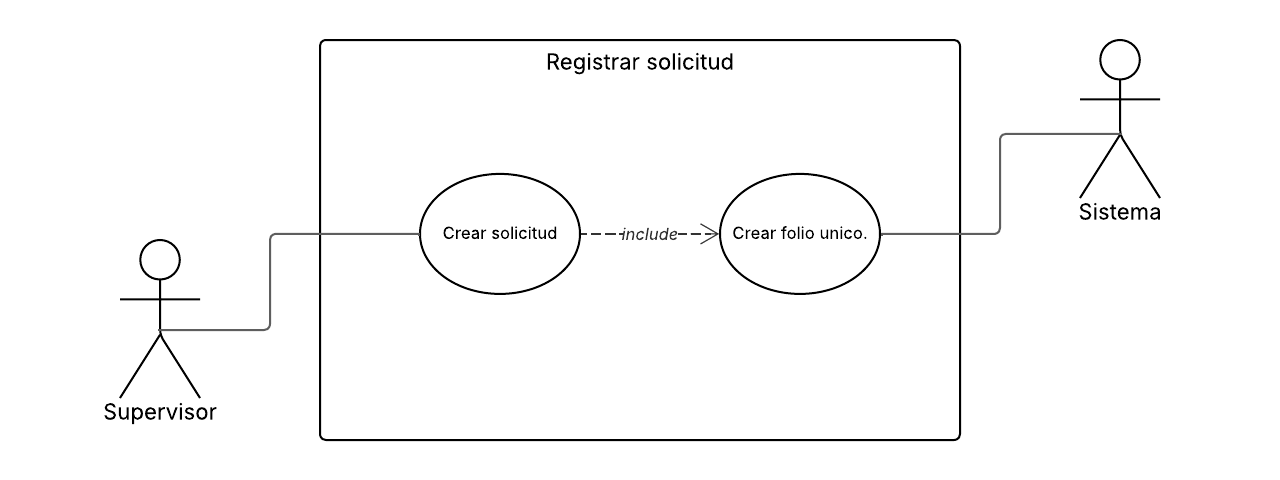
\includegraphics[width=0.9\textwidth]{DIACU01 (1).png}
  \caption{Caso de Uso 001}\label{d01}
\end{figure}

\begin{figure}[htp]
  \centering
  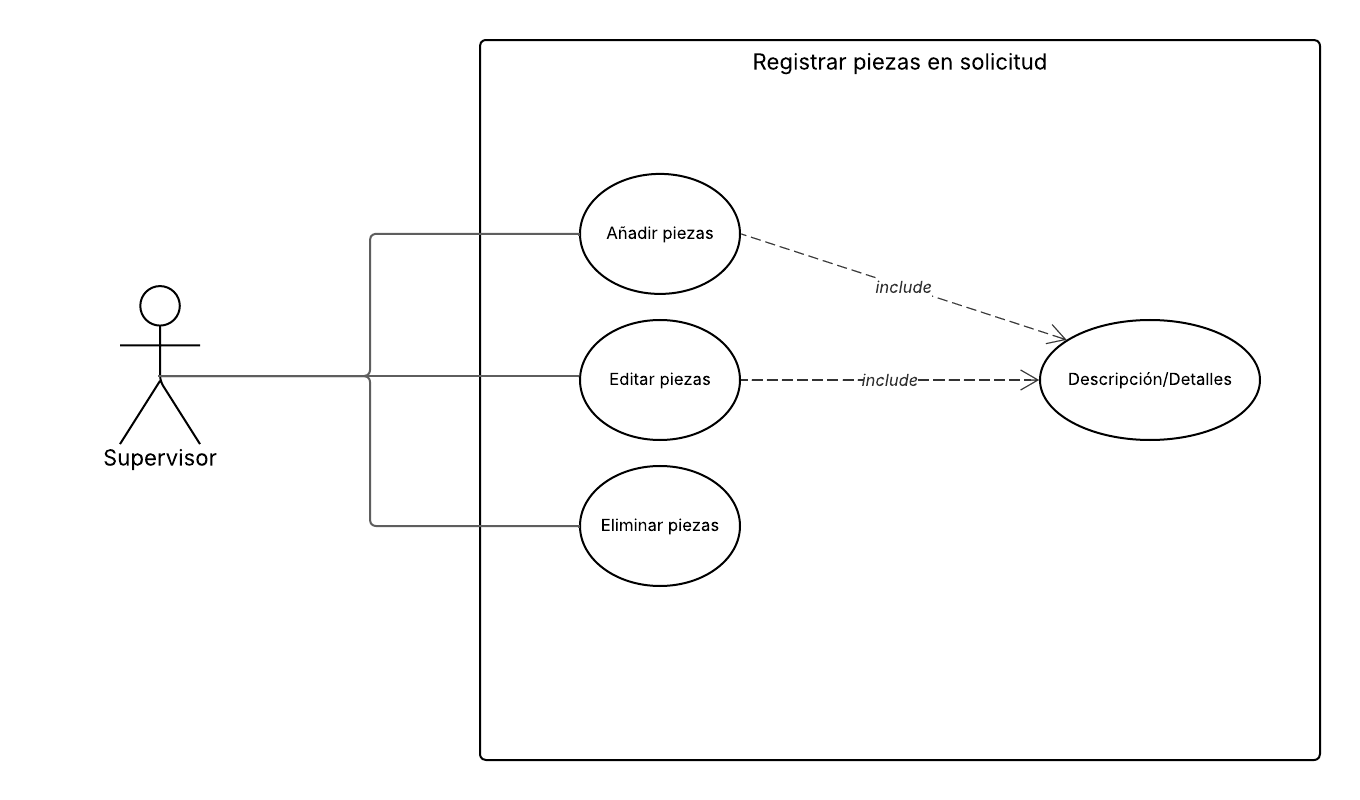
\includegraphics[width=0.9\textwidth]{DIACU02.png}
  \caption{Caso de Uso 002}\label{d02}
\end{figure}

\begin{figure}[htp]
  \centering
  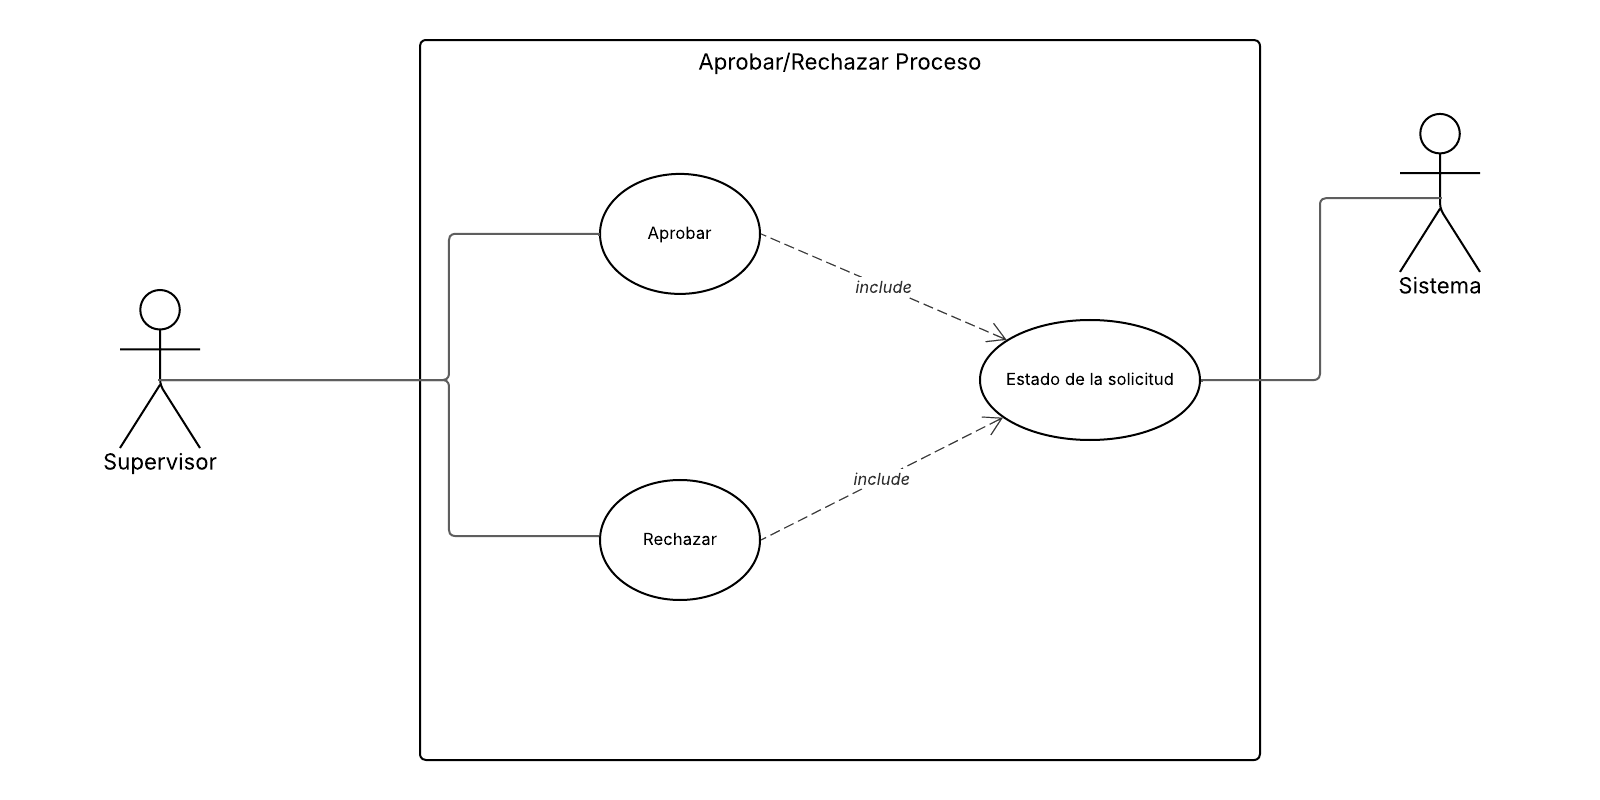
\includegraphics[width=0.9\textwidth]{DIACU03.png}
  \caption{Caso de Uso 003}\label{d03}
\end{figure}

\begin{figure}[htp]
  \centering
  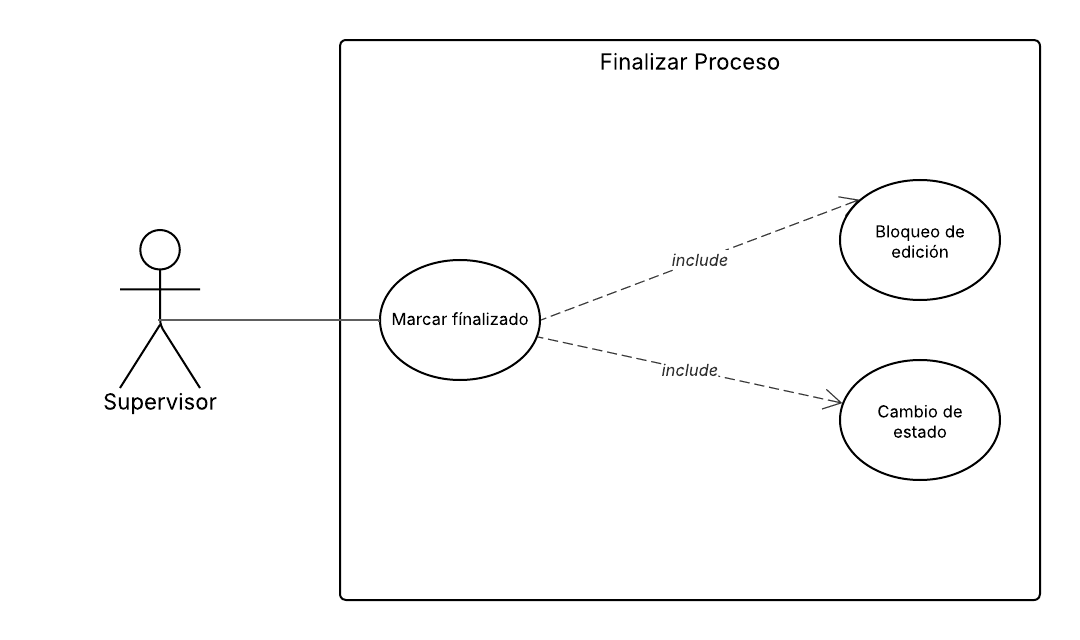
\includegraphics[width=0.9\textwidth]{DIACU04.png}
  \caption{Caso de Uso 004}\label{d04}
\end{figure}

\begin{figure}[htp]
  \centering
  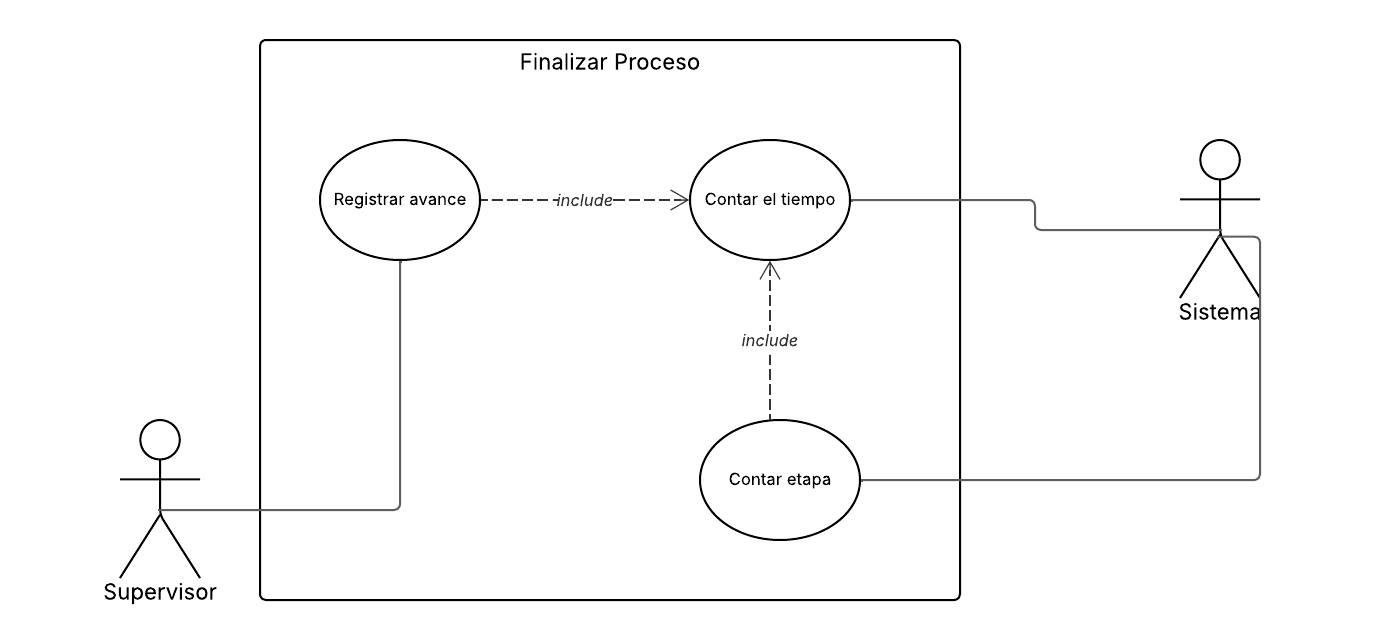
\includegraphics[width=0.9\textwidth]{DIACU05.png}
  \caption{Caso de Uso 005}\label{d05}
\end{figure}

\begin{figure}[htp]
  \centering
  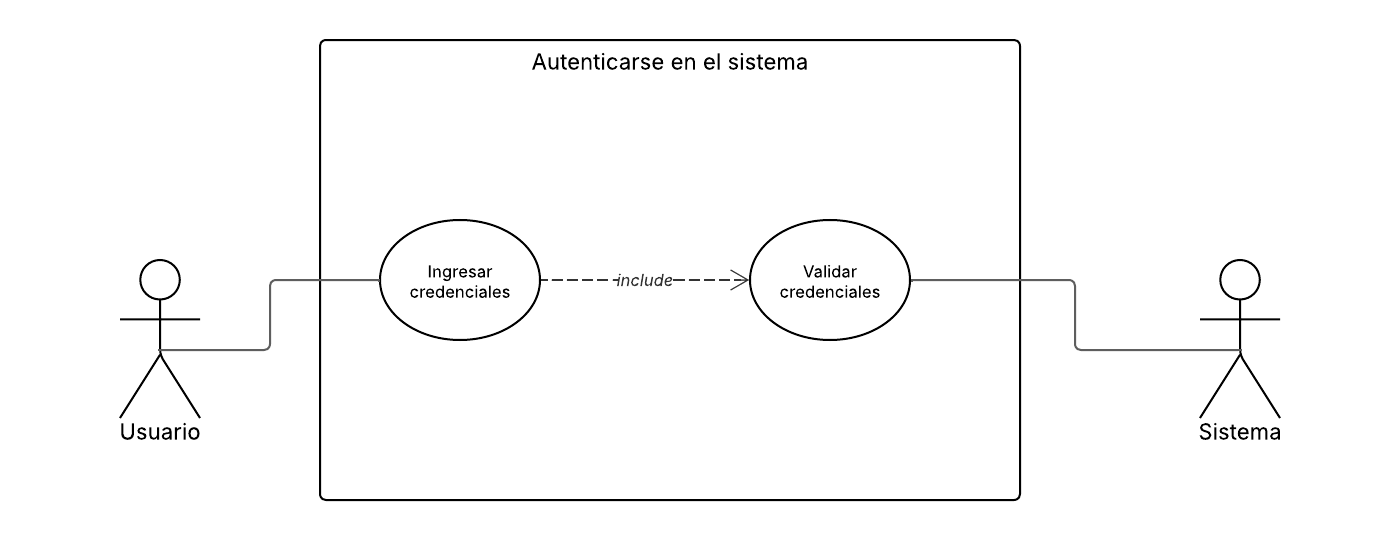
\includegraphics[width=0.9\textwidth]{DIACU06.png}
  \caption{Caso de Uso 006}\label{d06}
\end{figure}

\section{Implementación}

\section{Pruebas}


% CAPITULO RESULTADOS(estatus del proyecto y posibles mejoras) Y CONCLUSIONES(problemas presentados, costos, restrasos, cumplimiento de objetivos, etc)
%____________________________________________________________________________________________________________________

\chapter{Resultados y Conclusiones}
\newpage

\section{Resultados}


\section{Conclusiones}


% --------------------------  ANEXOS
%____________________________________________________________________________________________________________________

\newpage

% APENDICE O ANEXO (infoemacion adicional que se quiera anexar o agregar
% BIBLIOGRAFIA
\appendix

\nocite{book}
\nocite{dura2022saas}
\nocite{pretell2024mejora}
\nocite{odooDocs}
\nocite{book}


%\chapter{Bibliograf\check{}ía}
%\bibliographystyle{apalike}
%\bibliographystyle{unsrtnat}

% Eliminar la lista de ítems ficticios para evitar referencias no definidas.

\bibliographystyle{apalike}
\bibliography{biblio}
%\begin{thebibliography}{1}

%\bibitem{monk2008}
%Ellen Monk and Bret J. Wagner.
%\newblock \emph{Concepts in Enterprise Resource Planning}.
%\newblock Course Technology, 3rd edition, January 2008.

%\end{thebibliography}


\newpage
\chapter{Glosario}

\begin{description}
  \item[Asesor Académico] Persona encargada de regañar a los alumnos
\end{description}

\begin{description}
  \item[ERP(Enterprise Resource Planning)]  Sistema integrado que permite coordinar y 
  optimizar procesos empresariales clave, como finanzas, recursos humanos, logística y producción. 

\end{description}
%Otro apendice



\end{document} 